\documentclass{report}
\title{\textsc{A Digital Signal Processing Report on \\ \Huge Image Steganography using LSB Matching}}
\author{{\bf By: Himanshu Sharma} \\ {\bf Roll Number: $1610110149$} \\ {\bf Dept. of Electrical Engineering (ECE)} \\\\ {\bf Shiv Nadar University,} \\ {\bf Gautam Buddh Nagar,  Greater Noida, Uttar Pradesh 201314} \\\\\\ \textsc{ Under the guidance of Professor Vijay K. Chakka}}
\date{}

\usepackage[margin=0.8in]{geometry}
\usepackage{graphicx}
\usepackage{float}
\usepackage{amsmath}


\begin{document}
\maketitle
\pagenumbering{gobble}
\renewcommand{\thesection}{\arabic{section}}
% include the paper here.
\section{Paper Comprehension}
{\it Image Steganography} is the art of hiding information inside a digital image. Steagnography does not restrict to only plain text but it includes text, video, audio and image hiding also. In this report, the author has restricted himself to text data type only. Even when doing text embedding, there are immense possible algorithms to choose from. The most popular among them is the LSB replacement or Least Significant Bit replacement. With this type of algorithm, the least significant bit of each pixel (only one channel out of the RGB pallete) is changed by a bit decided according to the message bit. Therefore, we should not expect much change in the image after data hiding because the least significant bit is changed. For example, lets take a blue channel with value of 145. In binary, it is equivalent of 10010001. If by some technique, the last bit is changed to 0, then the decimal equivalent would become 144, which does not change the image much. This is the power of LSB replacement. It basically relies on the fact that hiding message bits in the LSB of each pixel does not affect the image much, in fact, the image practically remains as it is. There are, however, techniques now in modern signal processing science which can detect that some data is hidden in the image or not, a field called {\it steganalysis}. A successful hiding algorithm would be that, that would allow high payload and still look similar to the original image. 

\subsection{LSB Matching}
In LSB matching, if the message bit does not match with the pixel's LSB, then $\pm 1$ is randomly added to that pixel value. Unlike LSB replacement, where the pixel's LSB is just replaced by the message bit, here, a set of conditions are used to modify the pixel. LSB Matching could not be detected using the techniques used to detect LSB replacement. However, now it has been proved that LSB matching acts like a low pass filter on the digital images and therefore, this fact is utilized to detect whether LSB matching is applied on an image or not. \par Usually, two consecutive pixels are taken alongwith two consecutive message bits. The consecutive pairs are chosen randomly based on the {\it pseudo-random number generator} (PRNG). If the LSB matching is used as it is, then any pixel could be chosen with every pixel pair having equal chances of being selected by the algorithm. This has a flaw. This type of approach makes it difficult to disguise a changed pixel to the pixel surrounding it. For example, if lot of pixels are changed in a close vicinity, then they could be easily identified if the region is light in color, like sky which is light blue in color. The paper chosen here tries to rectify this problem by chosing those pixels on the image which lie on the edges. Edges are usually sharper than the surrounding regions and therefore its not easy to identify the change in pixel color on the edges. Similar papers have already been published. All of them suggest to use what is called the {\it pixel-value difference} (PVD). \par In PVD, what we do is that when we try to hide a message bit in a pixel's LSB, the pixel value is compared with its neighbouring pixels. If the difference is large, then more bits can be accomodated in that region without them being easily identified. Why? Because if there is a large difference in the pixel values then on changing the pixel value will not generate any significant difference. For example, if a pixel that is to be modified has a value of 45 and it's neighbouring pixel has a value of 145, then the difference $\displaystyle \Delta = 145-45=100$. Now, if by some technique if this pixel value if changed to 46, then the difference would become $\displaystyle \Delta' = 145-46 = 99$. To a human eye, this difference is not accountable. PVD is a good approach, in fact, far more better that PRNG because it utilizes the fact that sharp changes can be used to hide the information. \par In both LSB replacement and LSB matching, a travelling order is generated using PRNG which also acts as a key for decoding the stego-image. In both of these algorithms, the LSB of the selected pixel becomes equal to the message bit. According to the algorithm, the if the two consecutive pixels are $x_{i}$ and $x_{i+1}$ and the consecutive message bits are $m_{i}$ and $m_{i+1}$, then the pixels are modified such that $x_{i}$ becomes $x_{i}^{'}$ and $x_{i+1}$ becomes $x_{i+1}^{'}$ and the following relation holds.
\begin{center}
$ \displaystyle LSB(x_{i}^{'})=m_{i} \textrm{ and } LSB \Big( \Big\lfloor{\frac{x_{i}^{'}}{2}}\Big \rfloor + x_{i+1}^{'} \Big) = m_{i+1}$
\end{center}
From experiments done by the authors of the paper it has been shown that even if the cover image has rough textures, it will still have smooth regions in every $5 \times 5$ non-overlapping blocks. So, if by any chance, a pixel is selected in that region for message hiding then it could be easily identified. This is what the paper aims to solve.

\subsection{Bit Planes}
We now come to a brief discussion on what is called the bit planes. Bit planes help us visualize the importance of the significant bits used to represent the images. They clearly display the fact that altering the LSB of pixels is less damaging to the original image than altering the MSB of the same original image. Before we discuss them in great detail, let me show an example. Suppose we have a cover image which is shown below.

\begin{figure}[H]
\centering
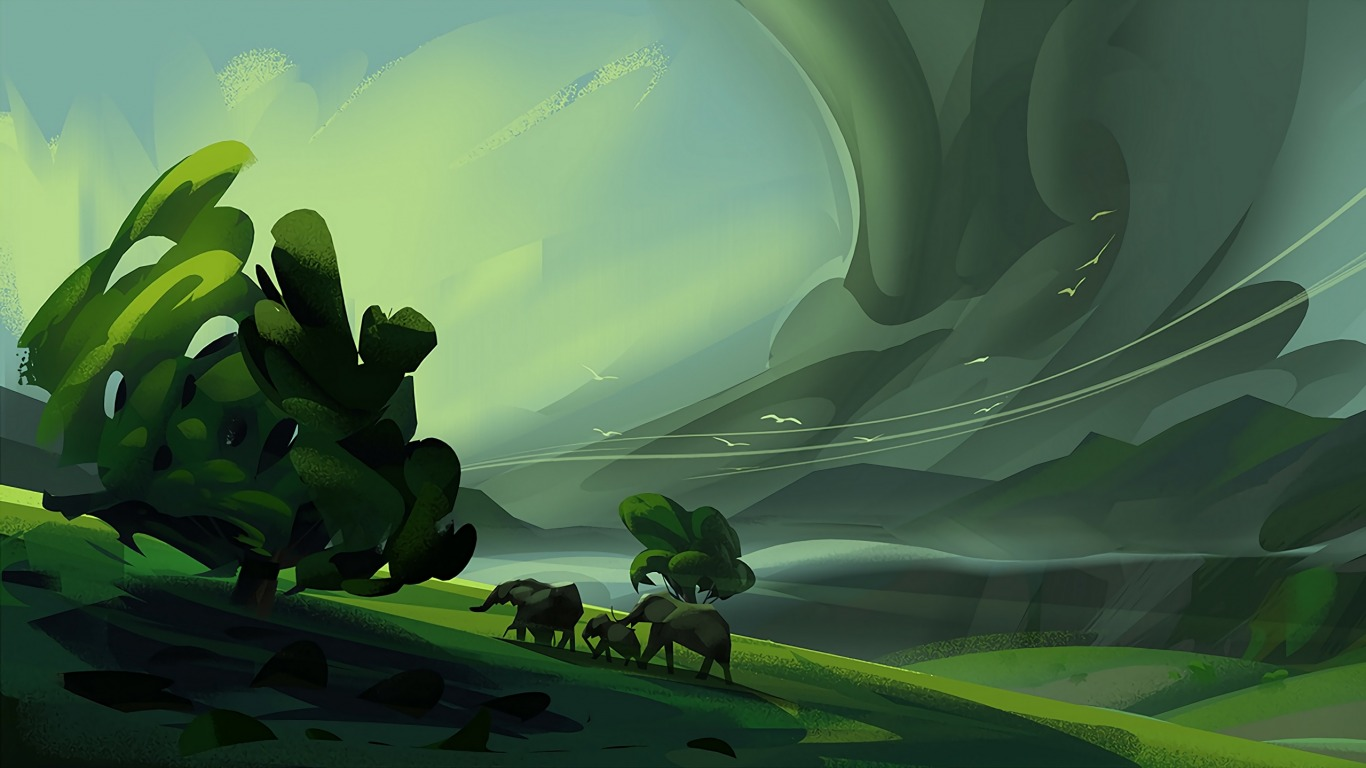
\includegraphics[width=0.5\textwidth]{images/desktop.jpg}
\caption{Cover Image}
\end{figure}
Its bit planes are shown below. The LSB plane and the MSB planes are what we display first.
\begin{figure}[H]
\centering
\begin{minipage}{0.46\linewidth}
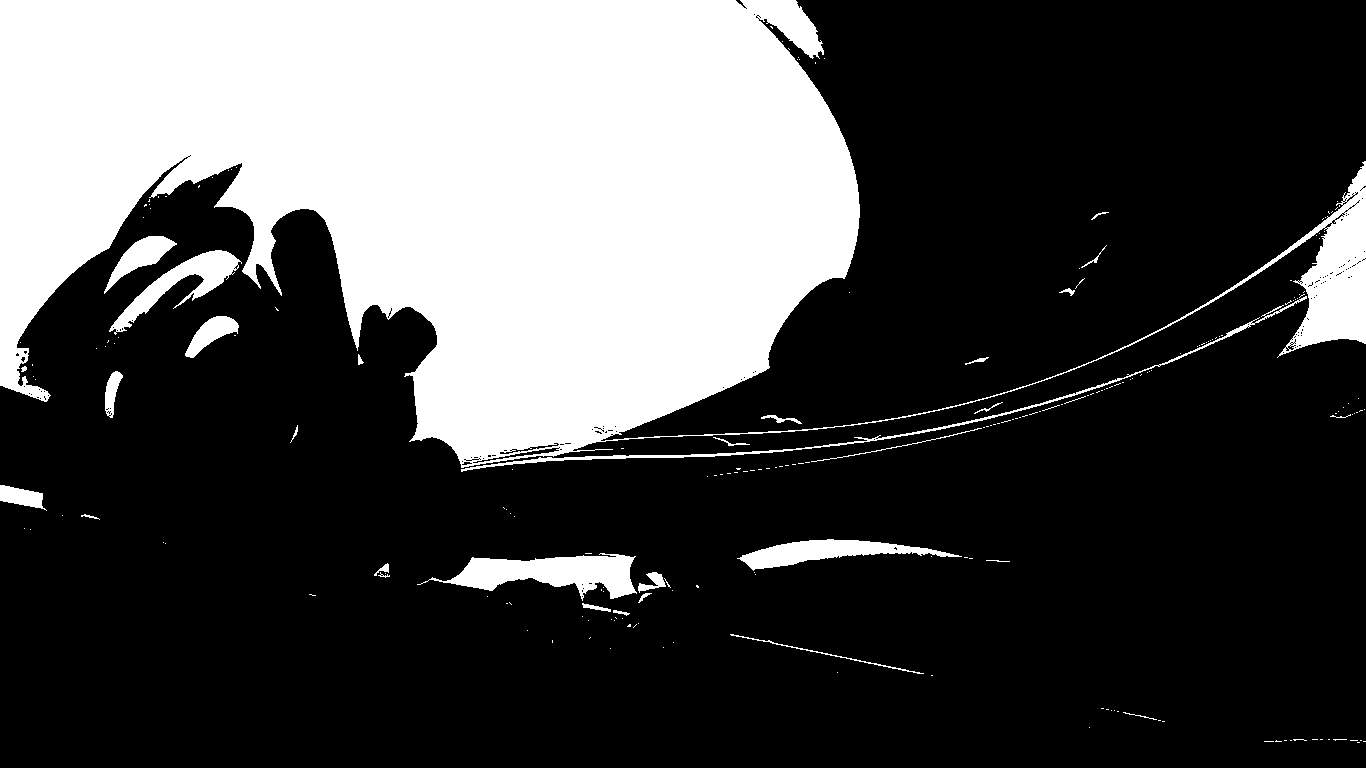
\includegraphics[width=\textwidth]{images/plane1.png}
\caption{MSB Plane}
\end{minipage}
\hfill
\begin{minipage}{0.46\linewidth}
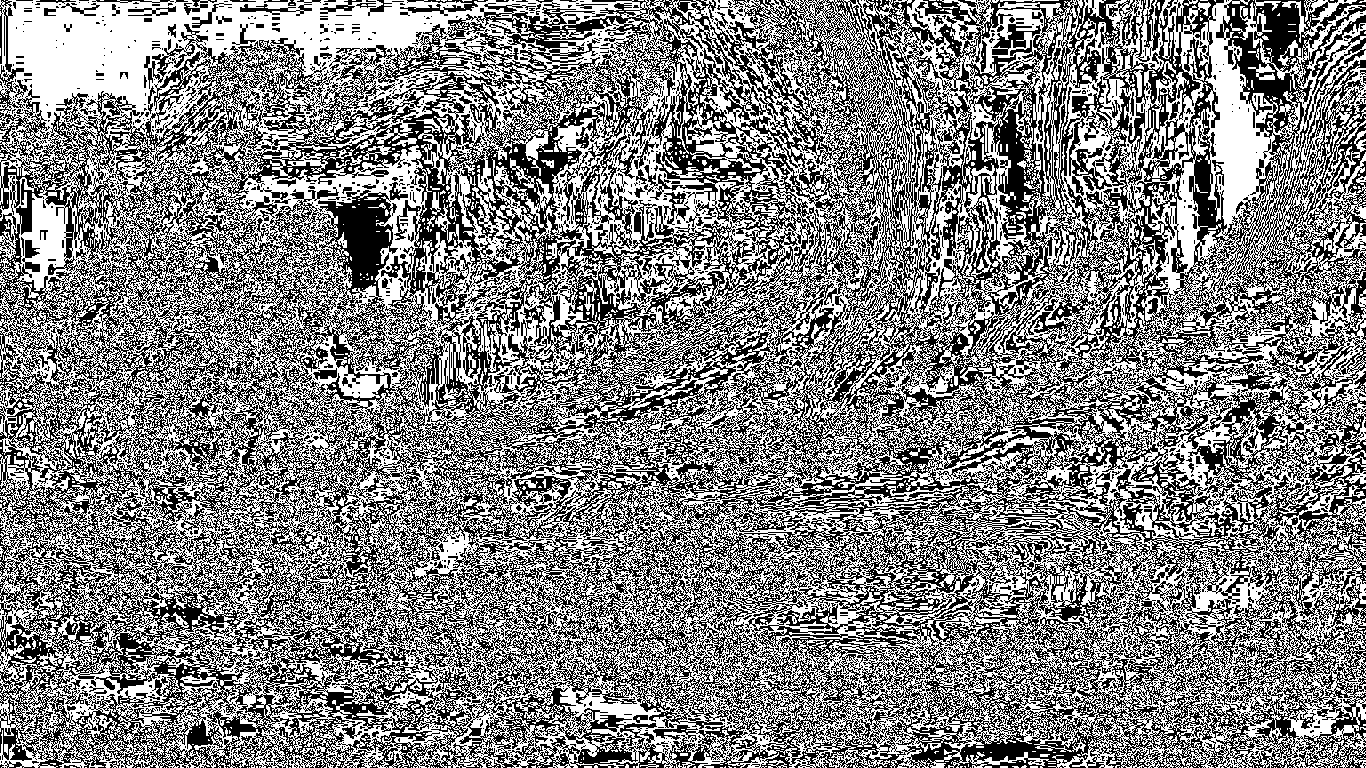
\includegraphics[width=\textwidth]{images/plane8.png}
\caption{LSB Plane}
\end{minipage}
\end{figure}

Changing a pixel value in the MSB plane is more prone to human eye detection as compared to the LSB plane. This is because a MSB plane has more structured black and white regions, and so, changing any pixel value, for example say, that a pixel is changed from white to black in the white region, then it would be easily detected. Whereas, on a LSB plane, the black and white regions are more uniformly aligned, just like {\it white noise} on a television screen. Inverting any color on the LSB plane won't change the visual effect. Hence, it is always advised to change the LSB plane in stegnography.
\par The idea is to generate these images using a single values. Since we have 3 values associated with a single pixel {\it (R, G, B)}, it would be a great idea to convert the image to a grayscale image, so that each pixel is represented by a single value. Now each pixel value, which initially was a three dimensional array, is converted to a one dimensional array having a single value. This matrix of single values (grayscale image) is passed to a function which converts these decimal pixel values to 8 bit binary number. As per the request of the user, the $i^{th}$ bit from each binary pixel is accessed. So, for example, if a pixel has 8-bit binary representation as 11110101 and the user asks for fifth bit plane, then the fifth bit from starting would be accessed and that is 0 for this example. These values are stored in another matrix. So now we have a matrix with only 1 and 0s. We now multiply each and every value of the matrix by 255. The matrix becomes full of 255 and 0s. Zero represent black color and 255 represent white color. When saved, this image is a black and white $i^{th}$ bit plane. 

\par Below, I have shown all the bit planes of the above cover image.
\begin{figure}[H]
\centering
\begin{minipage}{0.46\linewidth}
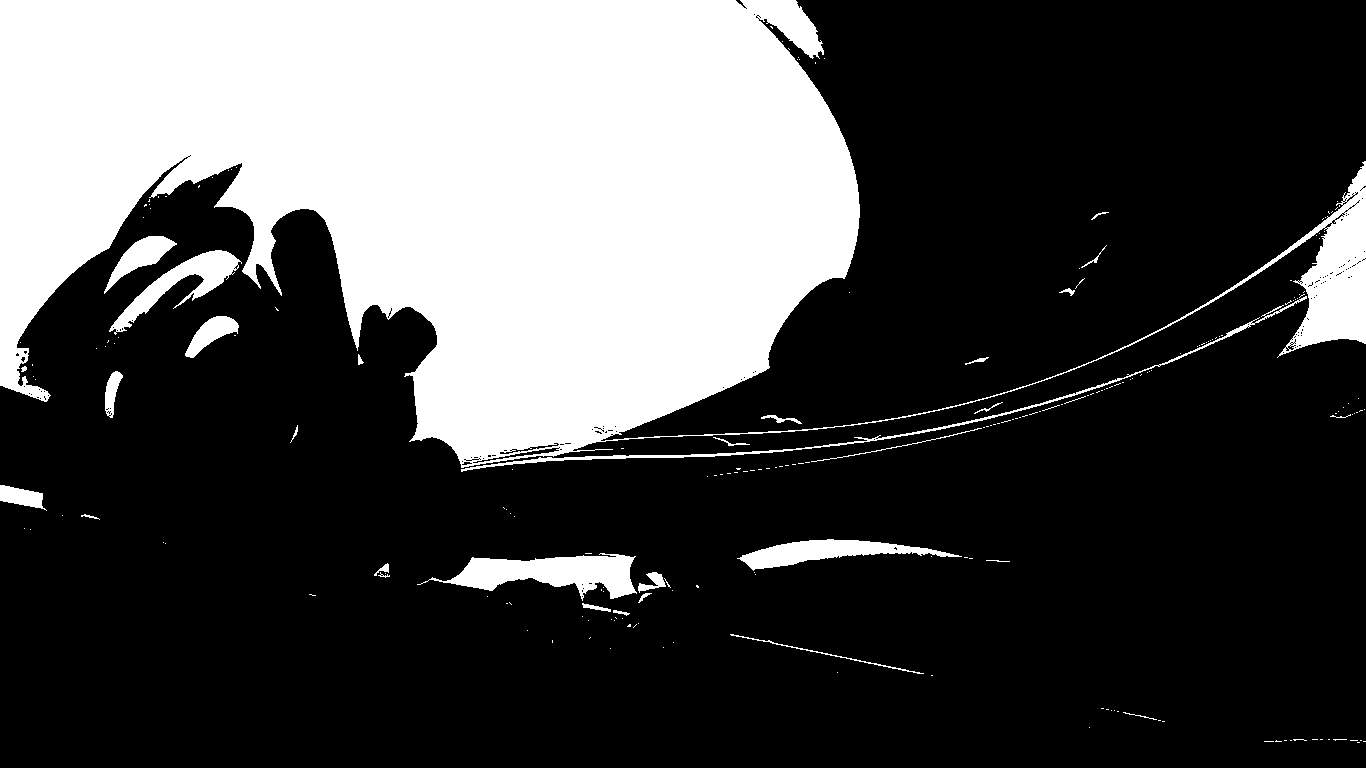
\includegraphics[width=\textwidth]{images/1.png}
\caption{$1^{st}$ bit plane or the MSB Plane}
\end{minipage}
\hfill
\begin{minipage}{0.46\linewidth}
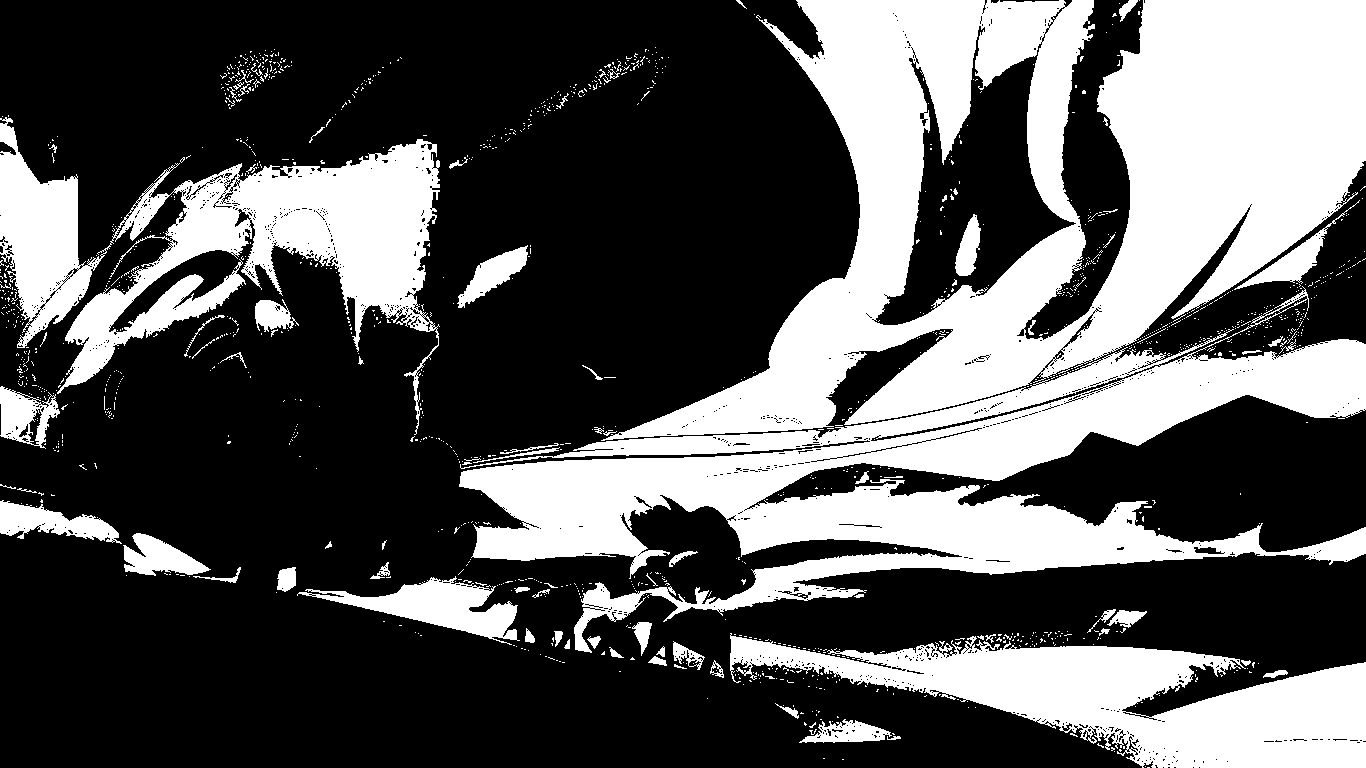
\includegraphics[width=\textwidth]{images/2.png}
\caption{$2^{nd}$ bit plane}
\end{minipage}
\vfill
\begin{minipage}{0.46\linewidth}
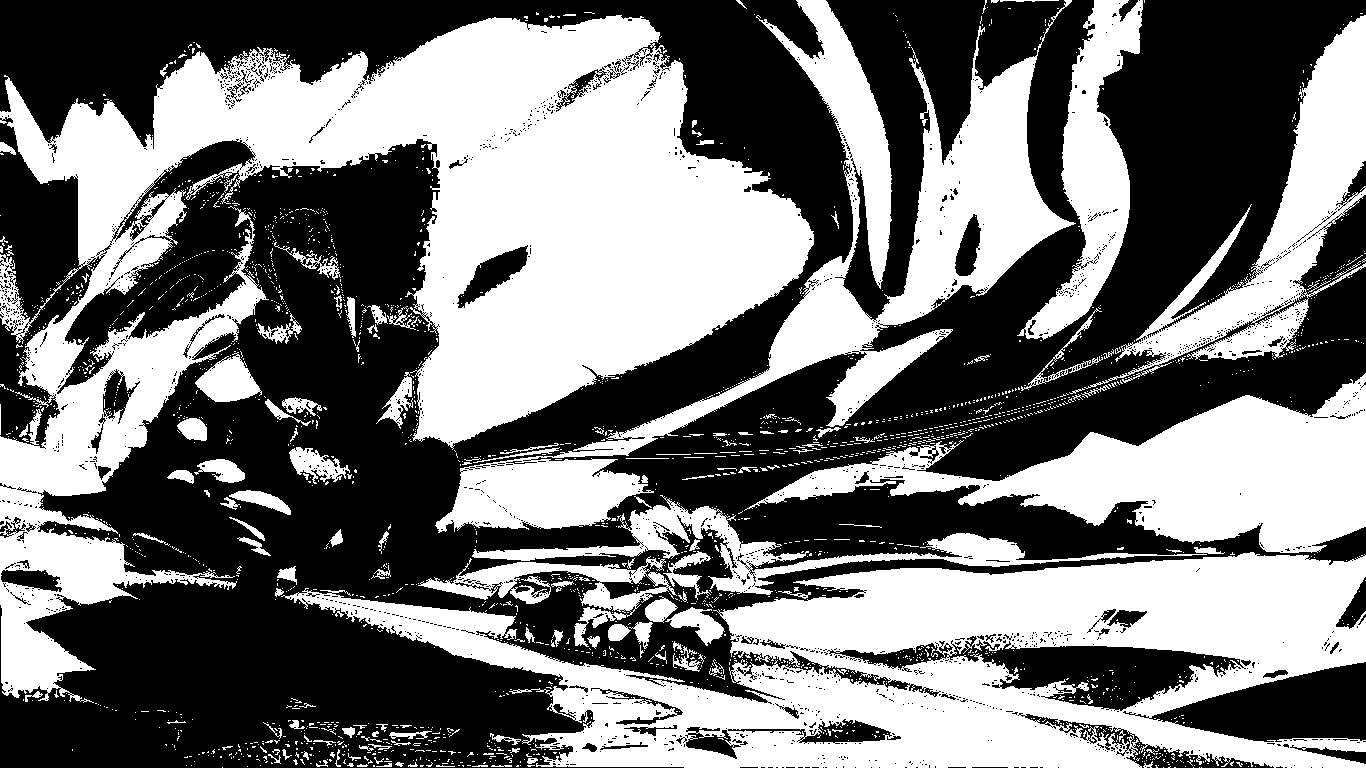
\includegraphics[width=\textwidth]{images/3.png}
\caption{$3^{rd}$ bit plane}
\end{minipage}
\hfill
\begin{minipage}{0.46\linewidth}
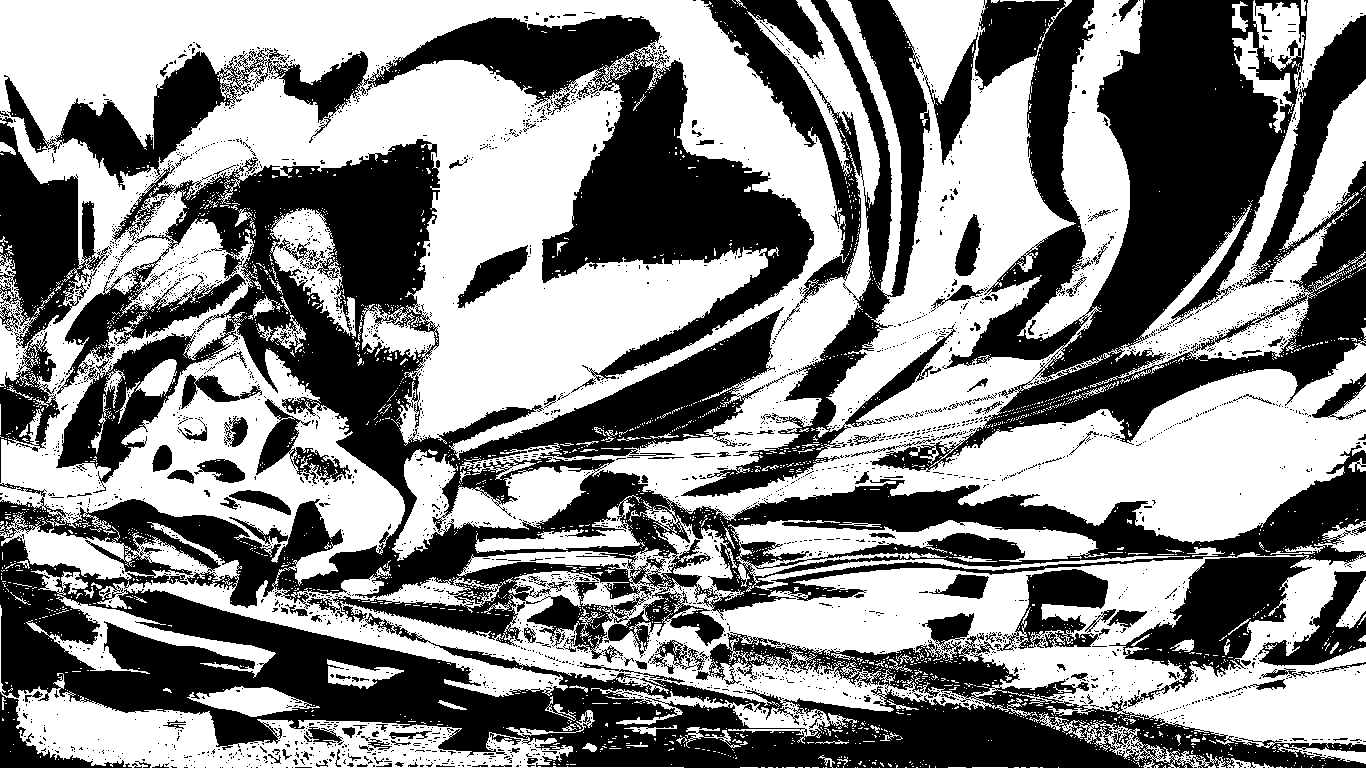
\includegraphics[width=\textwidth]{images/4.png}
\caption{$4^{th}$ bit plane}
\end{minipage}
\hfill
\begin{minipage}{0.46\linewidth}
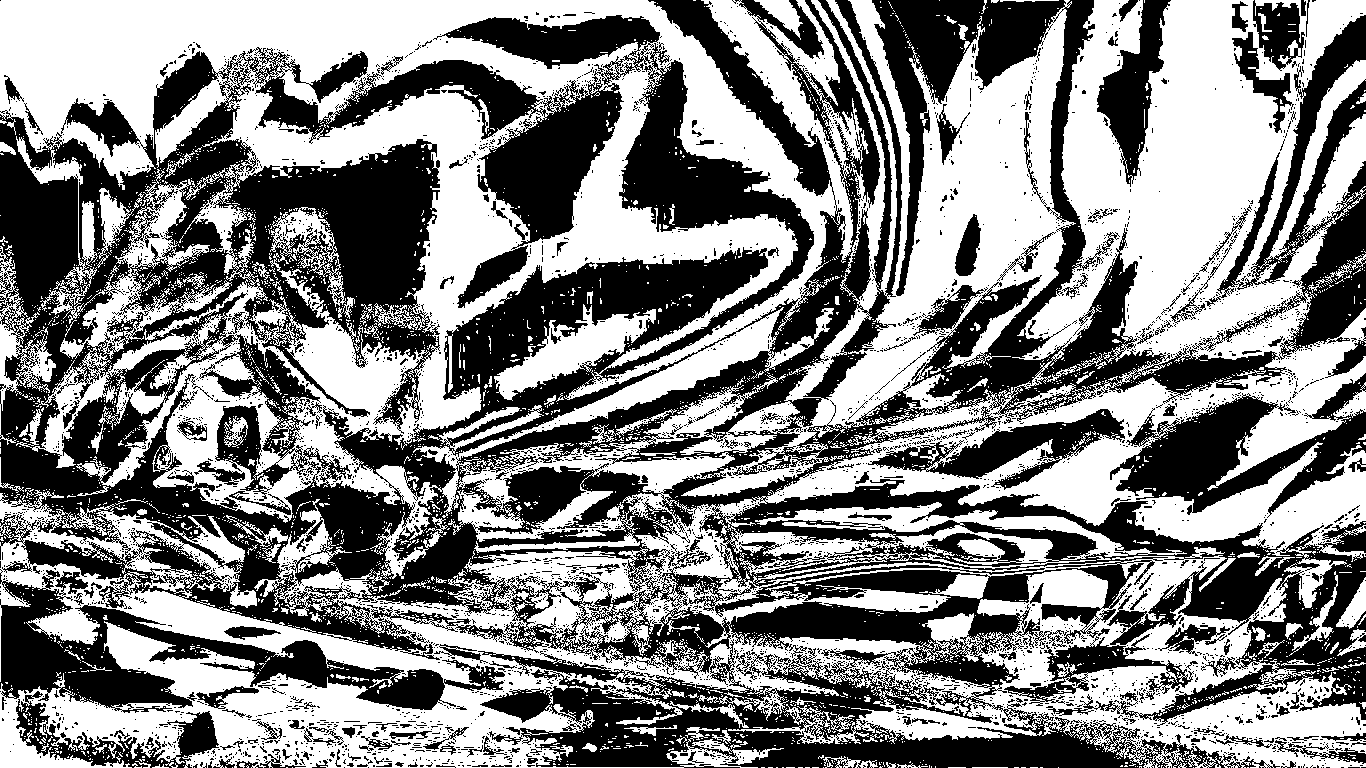
\includegraphics[width=\textwidth]{images/5.png}
\caption{$5^{th}$ bit plane}
\end{minipage}
\hfill
\begin{minipage}{0.46\linewidth}
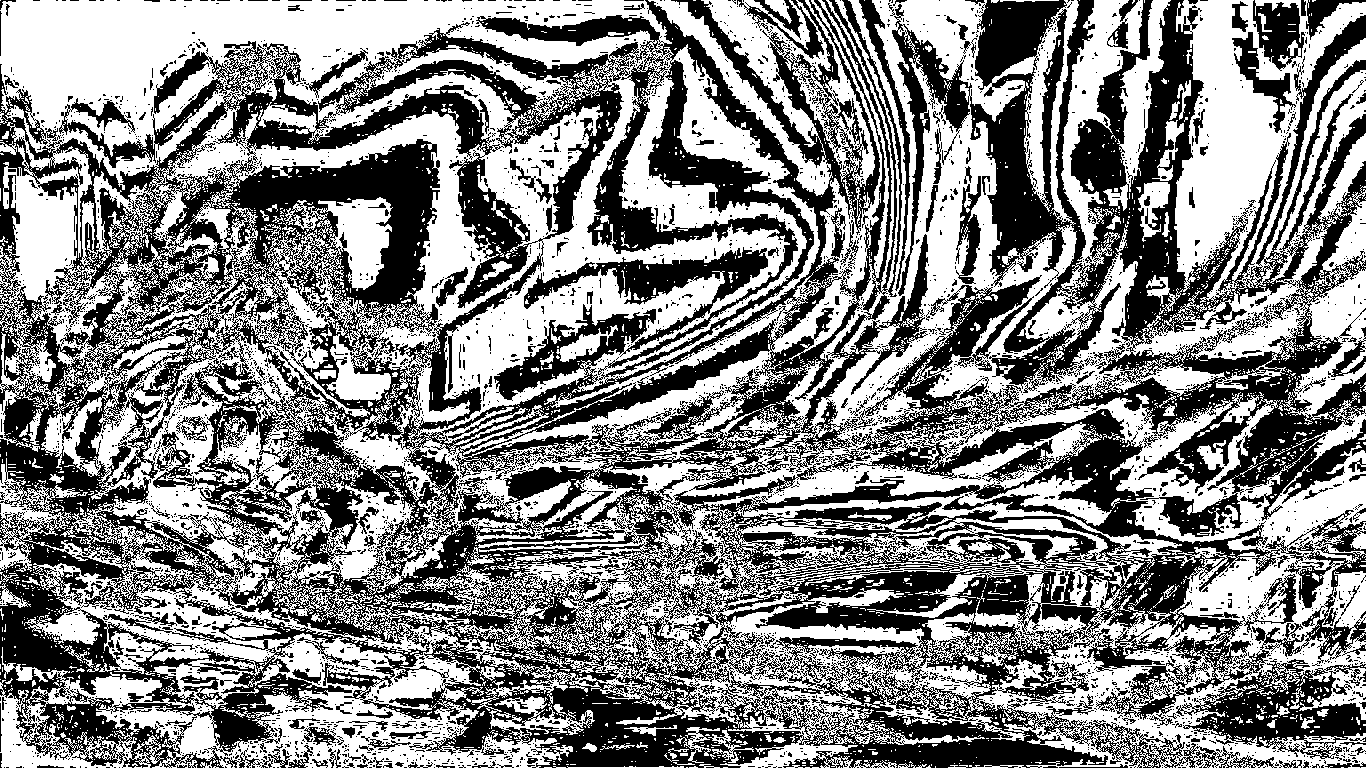
\includegraphics[width=\textwidth]{images/6.png}
\caption{$6^{th}$ bit plane}
\end{minipage}
\hfill
\begin{minipage}{0.46\linewidth}
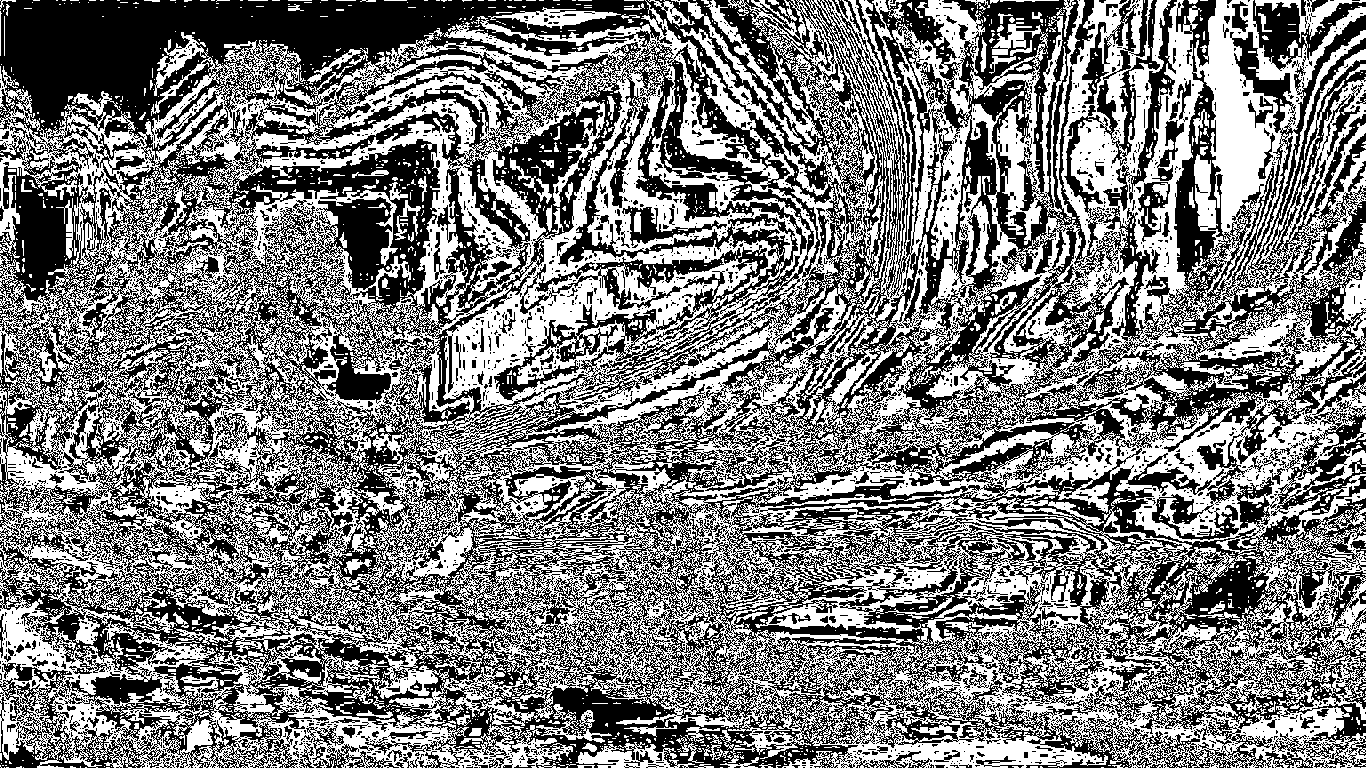
\includegraphics[width=\textwidth]{images/7.png}
\caption{$7^{th}$ bit plane}
\end{minipage}
\hfill
\begin{minipage}{0.46\linewidth}
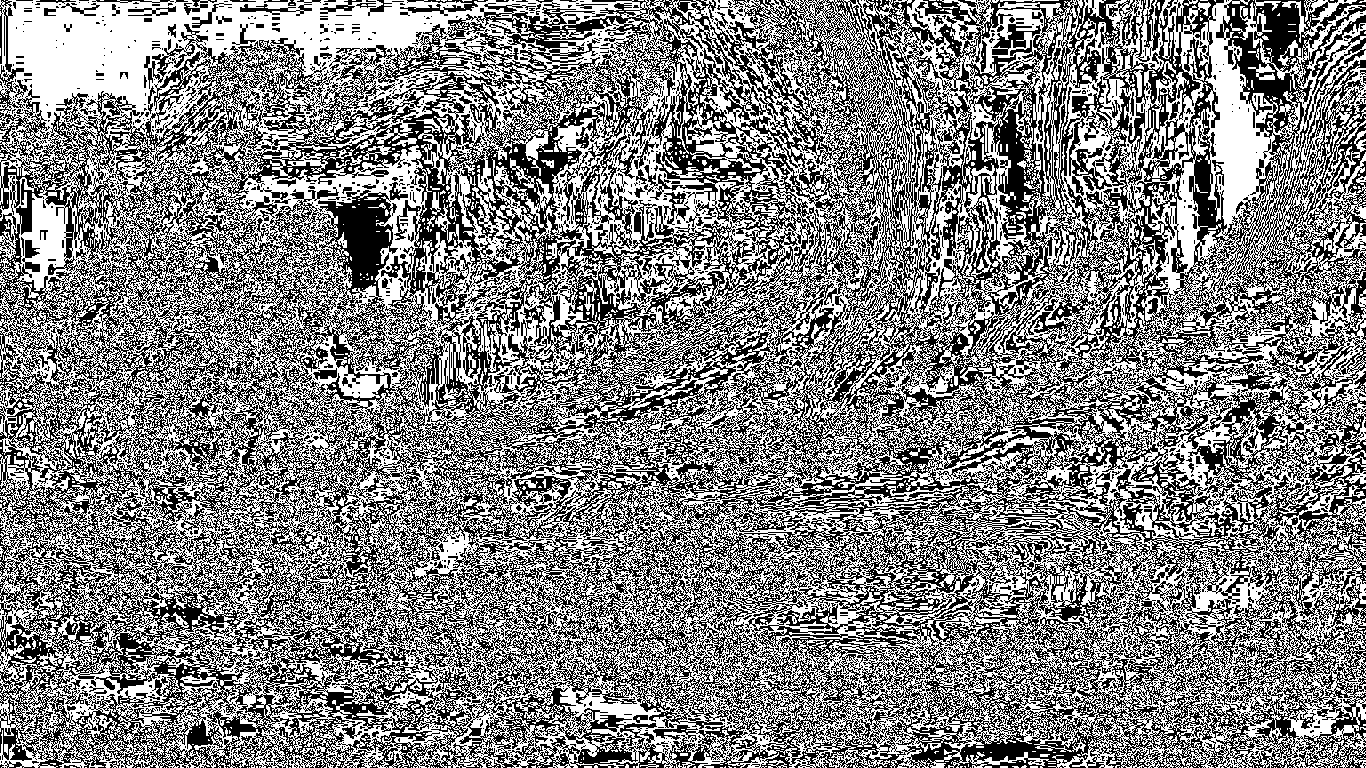
\includegraphics[width=\textwidth]{images/8.png}
\caption{$8^{th}$ bit plane or the LSB plane}
\end{minipage}

\end{figure}
Clearly, as we increase the bit plane number, we are bound to get more better results. Increasing the bit plane number implies less human eye detection in a pixel change. Now let us see the mathematical reasoning behind the bit planes. \newpage Let us define a closed form expression which converts a binary number to its decimal equivalent.
\begin{equation}
\displaystyle d(n) =\sum_{i=1}^{n}g(n+1-i,\textrm{ } b)2^{n-i}
\end{equation}
where $g(k, b)$ returns the $k^{th}$ bit from left of the binary number $b$ and $n$ denotes the length of the binary number. Here we are dealing with $n=8$. Let us say that the $j^{th}$ bit is changed while doing some steganography. The $j^{th}$ bit could be LSB or MSB or any other bit in between, we are not concerned about that for now. So, we know that $ 1 \leq j \leq n$. Let the original binary number be $\alpha$ and the binary number after the changed bit be denoted by $\beta$. Hence we get,

\begin{center}
$\displaystyle d_{1}(n) =\sum_{i=1}^{n}g(n+1-i,\textrm{ } \alpha)2^{n-i}$ and
$\displaystyle d_{2}(n) =\sum_{i=1}^{n}g(n+1-i,\textrm{ } \beta)2^{n-i}$
\end{center}
If we take the difference $\Delta d(n) = (d_{1} - d_{2})(n)$, the we get,
\begin{equation}
\displaystyle \Delta d(n) =\sum_{i=1}^{n}g(n+1-i,\textrm{ } \alpha)2^{n-i} - \sum_{i=1}^{n}g(n+1-i,\textrm{ } \beta)2^{n-i}
\end{equation}
Assuming all other bits of $\alpha$ and $\beta$ to be same except for the $j^{th}$ bit, we get,
\begin{center}
$\displaystyle \Delta d(n) = g(n+1-j, \alpha)2^{n-j} - g(n+1-j, \beta)2^{n-j} = 2^{n-j} \Delta g(n, j)$ 
\end{center}
where, $\Delta g(n, j) = g(n+1-j, \alpha) - g(n+1-j, \beta)$ and thus we get,
\begin{equation}
\displaystyle \delta (n) = |\Delta d(n)| = 2^{n-j}|g(n, j)|
\end{equation}

Note that $\Delta d(n)$ is the difference in the decimal values of the binary numbers which can be positive, negative or 0, $\delta (n)$ is always non-negative. Now, $|\Delta g(n, j)|$ can be defined as follows;
\[
|\Delta g(n, j)| = 
\begin{cases}
1, & j^{th} \text{ bit of $\alpha$ and $\beta$ are different} \\
0, & \text{otherwise}
\end{cases}
\]
The {\it otherwise} case is trivial because if there is no difference in even the $j^{th}$ bit of these binary numbers, then both of them are identical. This means that the number was not changed. But if the number has change, then $|\Delta g(n, j)|$, for sure, is 1. Now, it is in this part we are concerned with the difference. We need to minimize this difference $\delta(n)$ because then only our stego-image will be statistically close to the original image. The value of $\delta(n)$ could be minimum only if $n=j$ (see equation 3), i.e., $\delta(n) = |\Delta g(n, j)|$ which is 1 if we assume that the pixel bit was changed. That is, the difference in decimal value has the minimum magnitude of 1, 0 being the trivial case that the binary numbers were never changed. Since the decimal difference value will decide the grayscale of the stego-image, we want to minimize it. This proves that if we want statistically similar features in the stego-image, we should take $j=n$, i.e., we should consider the LSB only, because that would affect the orignal decimal value by $\pm 1$ only. \par If we do consider $j=1$, then $\delta(n) = 2^{n-1} |\Delta g(n, 1)|$. Again, $\Delta g(n, 1) = \pm 1$ if we consider that the pixel value was changed. However, it is clear that $2^{n-1}$ will yield the maximum difference, and therefore, $j=1$ should never be taken, or, MSB should never be changed.

\end{document}